\documentclass[11pt,a4paper,DIV=12]{scrartcl}

\makeatletter
\def\input@path{{../../../}}
\makeatother

\usepackage[sexy]{evan}
% \usepackage[sexy]{../../../evan}

% Override environment "problem" agar hanya menampilkan angka
\makeatletter
\newtheoremstyle{justnumber}
  {8pt} % space above
  {8pt} % space below
  {\normalfont} % body font
  {} % indent amount
  {\color{blue!40!black}\bfseries} % head font
  {} % punctuation after head
  {0.5em} % space after head
  {\thmnumber{#2}.\thmnote{ (\small #3)}} % head spec (hanya angka dan note)

% Hapus definisi problem lama di dalam makeatletter agar @ terbaca
\let\problem\relax
\let\endproblem\relax
\let\c@problem\relax
\let\theproblem\relax
\makeatother

\theoremstyle{justnumber}
\newtheorem{problem}{}

\begin{document}
\title{Pretest Pembinaan OSK Matematika}
\author{MAN 1 Pasuruan}
\date{23 April 2025}
\maketitle
\noindent\textbf{Petunjuk pengerjaan:}
\begin{itemize}
  \item Waktu pengerjaan adalah 90 menit.
  \item Terdapat 10 soal yang terdiri dari 5 soal kemampuan dasar dan 5 soal kemampuan lanjutan.
  \item Nilai soal kemampuan dasar adalah {\color{green!70!black}$B=+2$}, {\color{red}$S=0$}, $K=0$.
  \item Nilai soal kemampuan lanjutan adalah {\color{green!70!black}$B=+4$}, {\color{red}$S=-1$}, $K=0$.
  \item Gunakan bolpoin untuk menulis jawaban, dan coretlah jawaban yang salah.
\end{itemize}

\section*{Kemampuan Dasar}
\begin{problem}[LMNAS 2020]
  Diberikan $N=123456789101213...202320242025$. Jika $3^x$ membagi habis $N$, maka nilai maksimum dari $x$ bilangan bulat nonnegatif adalah \dots
\end{problem}

\begin{problem}[AIME 2002]

  \noindent
  Diagram berikut menunjukkan dua puluh lingkaran kongruen yang disusun dalam tiga baris dan berada di dalam sebuah persegi panjang. Lingkaran-lingkaran tersebut saling bersinggungan dan juga menyinggung sisi-sisi persegi panjang seperti pada gambar. Perbandingan panjang sisi terpanjang persegi panjang terhadap sisi terpendeknya dapat dinyatakan dalam bentuk
  $
    \frac{1}{2}(\sqrt{p} - q)
  $
  dengan $p$ dan $q$ bilangan bulat positif. Tentukan nilai $p + q$.

  \begin{center}
    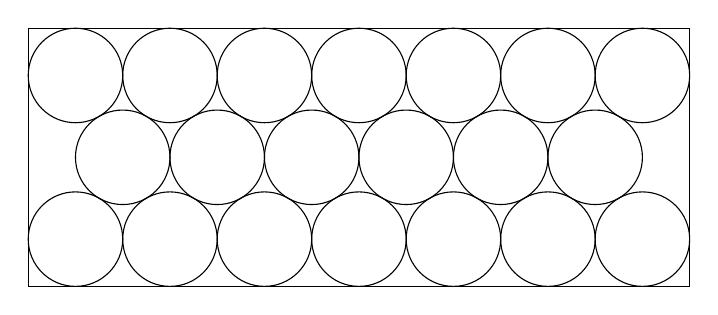
\begin{tikzpicture}[scale=0.6]

      % jari-jari
      \def\r{1}

      % Baris atas (7 lingkaran)
      \foreach \i in {0,...,6} {
          \draw ({2*\i*\r}, {\r + 1.5*sqrt(3)*\r}) circle (\r);
        }

      % Baris tengah (6 lingkaran, digeser)
      \foreach \i in {0,...,5} {
          \draw ({2*\i*\r + \r}, {\r + sqrt(3)*\r/2}) circle (\r);
        }

      % Baris bawah (7 lingkaran)
      \foreach \i in {0,...,6} {
          \draw ({2*\i*\r}, {\r- sqrt(3)*\r/2}) circle (\r);
        }

      % Persegi panjang pembungkus
      \draw ({-\r}, {-sqrt(3)*\r/2}) rectangle ({12*\r + \r}, {\r + 1.5*sqrt(3)*\r + \r});
    \end{tikzpicture}
  \end{center}
\end{problem}

\begin{problem}[KSN-K 2020]
  Misalkan $x, y$ bilangan asli sehingga $2x + 3y = 2020$. Nilai terbesar yang mungkin dari $3x + 2y$ adalah $\ldots$
\end{problem}

\begin{problem}[OSK 2019]
  Tujuh buah bendera dengan motif berbeda akan dipasang pada 4 tiang bendera. Pada masing-masing tiang bendera bisa dipasang sebanyak nol, satu, atau lebih dari satu bendera. Banyaknya cara memasang bendera tersebut adalah \dots
\end{problem}

\begin{problem}[OSP 2020]
  Sejumlah siswa mengikuti ujian dengan komposisi soal sebagai berikut:
  \begin{itemize}
    \item Bagian pertama terdiri dari 3 soal dengan dua pilihan (benar/salah)
    \item Bagian kedua terdiri dari 5 soal pilihan ganda dengan lima pilihan (A, B, C, D, E)
  \end{itemize}
  Banyaknya siswa minimal agar senantiasa terdapat dua siswa dengan jawaban sama persis baik pada bagian pertama maupun kedua adalah \dots
\end{problem}

\section*{Kemampuan Lanjutan}
\begin{problem}[OSK 2024]
  Untuk setiap bilangan real $x$, notasi $\lfloor x \rfloor$ menyatakan bilangan bulat terbesar yang kurang dari atau sama dengan $x$. Sebagai contoh $\lfloor 1{,}1 \rfloor = 1$, $\lfloor 3 \rfloor = 3$, dan sebagainya. Jika ada tepat sebanyak $1000$ bilangan berbeda pada barisan
  \[
    \left\lfloor \frac{1^2}{2024} \right\rfloor,\;
    \left\lfloor \frac{2^2}{2024} \right\rfloor,\;
    \left\lfloor \frac{3^2}{2024} \right\rfloor,\;
    \ldots,\;
    \left\lfloor \frac{n^2}{2024} \right\rfloor,
  \]
  maka $n = \ldots$
\end{problem}

\begin{problem}[KSN-K 2021]
  Diberikan segitiga $ABC$ dengan $AB = 6$, $BC = 7$, dan $CA = 8$. Jika $I$ adalah titik potong ketiga garis bagi segitiga $ABC$, maka $AI^2$ adalah $\ldots$
\end{problem}


\begin{problem}[OSK 2025]
  Perhatikan gambar berikut.

  \begin{center}
    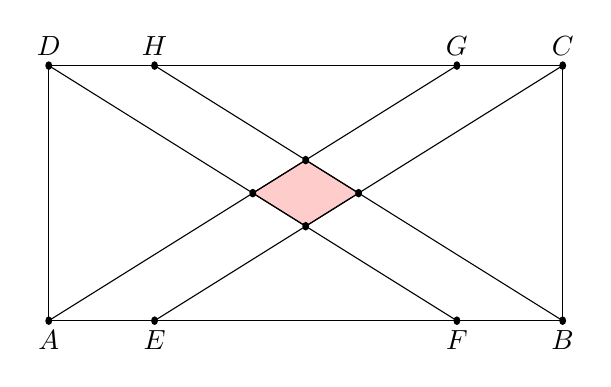
\begin{tikzpicture}[scale=0.12,xscale=0.8] % Skala disesuaikan agar pas di halaman
      % Koordinat titik sudut persegi panjang
      \coordinate (A) at (0,0);
      \coordinate (B) at (68,0);
      \coordinate (C) at (68,27);
      \coordinate (D) at (0,27);

      % Koordinat titik E, F pada AB dan G, H pada CD
      \coordinate (E) at (14,0);
      \coordinate (F) at (54,0);
      \coordinate (H) at (14,27);
      \coordinate (G) at (54,27);

      % Menghitung titik potong untuk daerah yang diarsir
      % Perpotongan AG dan DF
      \coordinate (I1) at (27, 13.5);
      % Perpotongan AG dan BH
      \coordinate (I2) at (34, 17);
      % Perpotongan CE dan BH
      \coordinate (I3) at (41, 13.5);
      % Perpotongan CE dan DF
      \coordinate (I4) at (34, 10);

      % Menggambar dan mewarnai daerah yang diarsir
      \fill[pink!80] (I1) -- (I2) -- (I3) -- (I4) -- cycle;

      % Menggambar garis pinggir daerah arsir (opsional, untuk mempertegas)
      \draw (I1) -- (I2) -- (I3) -- (I4) -- cycle;

      % Menggambar persegi panjang dan garis-garis silang
      \draw (A) -- (B) -- (C) -- (D) -- cycle;
      \draw (A) -- (G);
      \draw (B) -- (H);
      \draw (C) -- (E);
      \draw (D) -- (F);

      % Menggambar titik-titik (menggunakan ukuran absolut 'pt' agar tidak terpengaruh scale)
      \foreach \p in {A,B,C,D,E,F,G,H,I1,I2,I3,I4}{
          \fill (\p) circle (13pt);
        }
      % Label titik-titik
      \node[below] at (A) {$A$};
      \node[below] at (B) {$B$};
      \node[above] at (C) {$C$};
      \node[above] at (D) {$D$};
      \node[below] at (E) {$E$};
      \node[below] at (F) {$F$};
      \node[above] at (G) {$G$};
      \node[above] at (H) {$H$};
    \end{tikzpicture}
  \end{center}
  Diketahui persegi panjang $ABCD$ dengan titik $E, F,$ pada $AB$ dan $G, H$ pada $CD$ sehingga $AF = BE = CH = DG = 54$. Jika $AB = 68$ dan $AD = 27$, maka luas daerah yang dibatasi oleh $AG, CE, BH,$ dan $DF$ adalah ....
\end{problem}


\begin{problem}[OSK 2024]
  Diberikan suku banyak $P(x) = x^3 + Dx^2 + Ex + 1$ dan $P(-1) = 4$. Jika $a, b, c$ merupakan akar-akar dari $P(x) = 0$ dan memenuhi $(a^2 - bc)(b^2 - ca)(c^2 - ab) = 40$. Maka nilai dari $(D + E)^2$ adalah \dots
\end{problem}

\begin{problem}[OSK 2022]
  Banyaknya tripel $(w_1, w_2, w_3, \dots, w_7)$ yang memenuhi persamaan
  \[ w_1 + w_2 + w_3 + \dots + w_7 = 148 \]
  dengan $20 \leq w_1, w_2, w_3, \dots, w_7 \leq 22$ adalah \dots
\end{problem}
\end{document}